\section{Intelligenza Artificiale}

\begin{figure}
    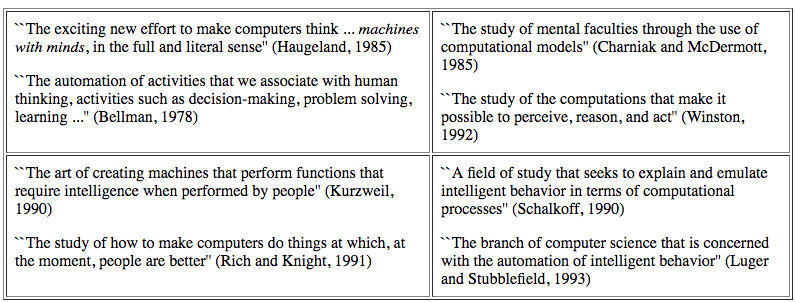
\includegraphics[width=\linewidth]{aidef}
    \caption{Possibili definizioni di Intelligenza artificiale\cite{aima}}
    \label{fig:ai}
  \end{figure}
Dare un'unica definizione di intelligenza artificiale risulta estremamente difficile a causa della vastità
e dell'interdisciplinarietà dell'argomento. Soltanto nella figura \ref{fig:ai} ne troviamo addirittura otto, tutte valide, ma forse
la descrizione  migliore per i nostri scopi  è quella data dal padre di questa disciplina, John Mccarthy:
'' L'Intelligenza Artificiale è la scienza volta alla creazione di macchine  \emph{intelligenti},
più nello specifico di \emph{programmi intelligenti}.'' \cite{ai}.
\subsection{Agenti e ambienti}
Il concetto di macchina intelligente può essere ulteriormente
astratto dall'idea di \textbf{agente computazionale intelligente}. Esaminiamo adesso questa definizone.
Un \textbf{agente} è un'entità che compie azioni
e percepisce informazioni da un ambiente.

\begin{figure}
  \centering
  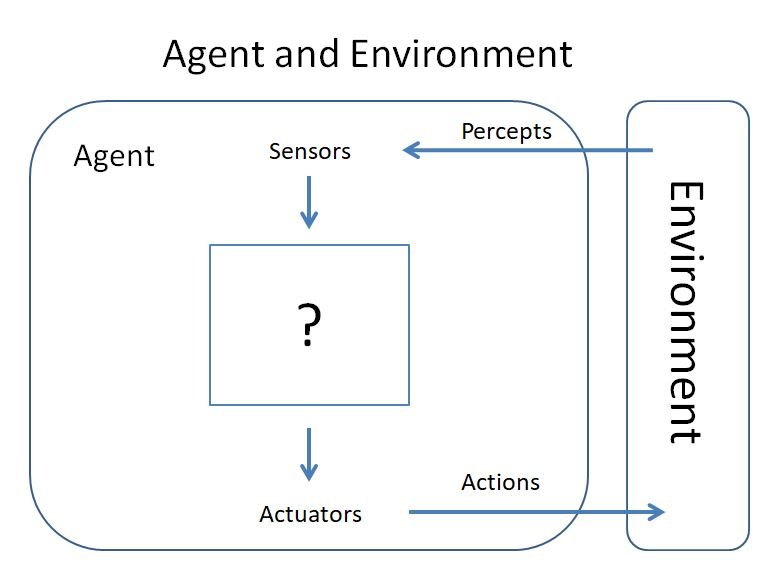
\includegraphics[scale=0.4]{agent}
  \caption{Agente computazionale\cite{aima}}
  \label{fig:agente}
\end{figure}

Un'agente si comporta in modo \textbf{intelligente} quando:
\begin{itemize}
  \item le sue azioni sono appropriate alle circostanze e ai suoi scopi
  \item È flessibile per ambienti e scopi dinamici
  \item impara dall'esperienza
  \item fa le scelte \textbf{giuste} date le sue limitazioni percettive e computazionali. Un agente tipicamente
  non può osservare l'ambiente direttamente; ha una memoria e un tempo per agire molto limitati.
\end{itemize}
 Un agente \textbf{computazionale} è un agente le cui decisioni possono essere descritte in termini di una
 computazione. Questo significa che una decisione può essere scomposta in una serie di operazioni primitive
 implementabili in un dispositivo fisico \cite{PooleMackworth17}.
 \subsection{Intelligenza e performance}
 Abbiamo detto che un agente è intelligente quando compie le \emph{scelte giuste}. Ma cosa significa fare la scelta giusta?
 Rispondiamo a questa domanda in un modo molto banale: considerando le \emph{consequenze} del comportamento di un agente.
 Un agente si muove all'interno di un ambiente e compie una sequenza di azioni in base alle informazioni che riceve.
 Queste azioni causano variazioni allo stato dell'ambiente. Se la variazioni è desiderabile, l'agente ha fatto le scelte giuste.
 La nozione di desiderabilità è catturata da una \textbf{misura di prestazione (performance measure)} che valuta una qualunque sequenza di azioni.
 Ovviamente non esiste una performance measure globale; solitamente viene costruita appositamente  per uno specifico problema.
 Le specifiche dell'agente, dell'ambiente e della misura di prestazioni vengono raggruppate nell'\textbf{ambiente di lavoro (task environment)},
 attraverso la descrizione PEAS (Performance,Environment,Actuators,Sensors)\cite{aima}.
 \begin{figure}
  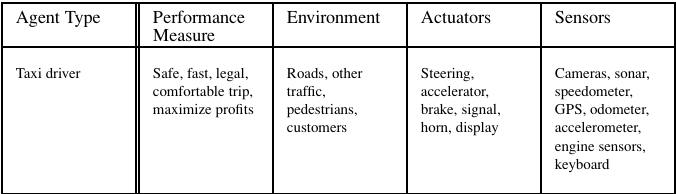
\includegraphics[width=\linewidth]{peas_taxi.png}
  \caption{descrizione PEAS dell'ambiente di lavoro di un taxi automatico\cite{aima}}
  \label{fig:taxi}
 \end{figure}
 La figura \ref{fig:taxi} riassume un esempio di descrizione PEAS dell'ambiente di lavoro di un taxi.
\subsection{Razionalità}
Ciò che abbiamo descritto fin'ora ci permette di verificare in modo quantitativo l'intelligenza di un agente.
Espandiamo questa idea introducendo la nozione di \textbf{razionalità}.
Cosa sia razionale in qualsiasi momento dipende da quattro elementi:
\begin{itemize}
  \item la misura di prestazioni;
  \item la conoscenza a priori dell'agente;
  \item le azioni che l'agente può compiere;
  \item la sequenza di percezioni fino a quel momento.
\end{itemize}
Questo ci porta alla definizione di \textbf{Agente Razionale}:
      \begin{center}
      \emph{per ciascuna sequenza di percezioni, un agente razionale seleziona un'azione che massimizza il valore atteso della performance measure, data l'evidenza 
      fornita dalla sequenza di percezioni e dalla conoscenza a priori dell'agente}
      \end{center}
La razionalità non significa \textbf{onniscienza}. Un agente deve essere in grado di prendere decisioni anche quando
non ha a disposizione tutte le informazioni necessarie a compiere l'azione perfetta. Un agente razionale massimizza \emph{il valore atteso} della performance
basandosi sulla sua conoscenza pregressa dell'ambiente, ma  non sempre un ambiente è completamente osservabile. Per questo motivo sono
fondamentali la fase di raccolta delle informazioni (\textbf{information gathering}) e di apprendimento (\textbf{learning}). Per poter
migliorare le prestazioni, un  agente deve essere in grado di raccogliere la massima quantità possibile di informazioni
e di aggiungere tali informazioni alla propria base di conoscenza. Questo permette una scelta sempre migliore delle azioni da compiere \cite{aima}.
\subsection{Scopo dell'IA}
Lo scopo scientifico  dell'IA è quello di studiare i principi e i meccanismi che rendono il comportamento intelligente possibile sia
nei sistemi naturali che in quelli artificiali. Lo scopo ingegneristico di questa disciplina è la costruzione di dispositivi fisici
in grado di comportarsi in modo intelligente. Da queste basi si sono sviluppati un innumerevole quantità di branche, tra cui le più importanti sono \cite{ai}:
\begin{itemize}
  \item \textbf{logical AI}
  \item \textbf{search}
  \item \textbf{knowledge and reasoning}
  \item \textbf{planning}
  \item \textbf{learning from experience}
  \item \textbf{genetic programming}
\end{itemize}
\begin{figure}
  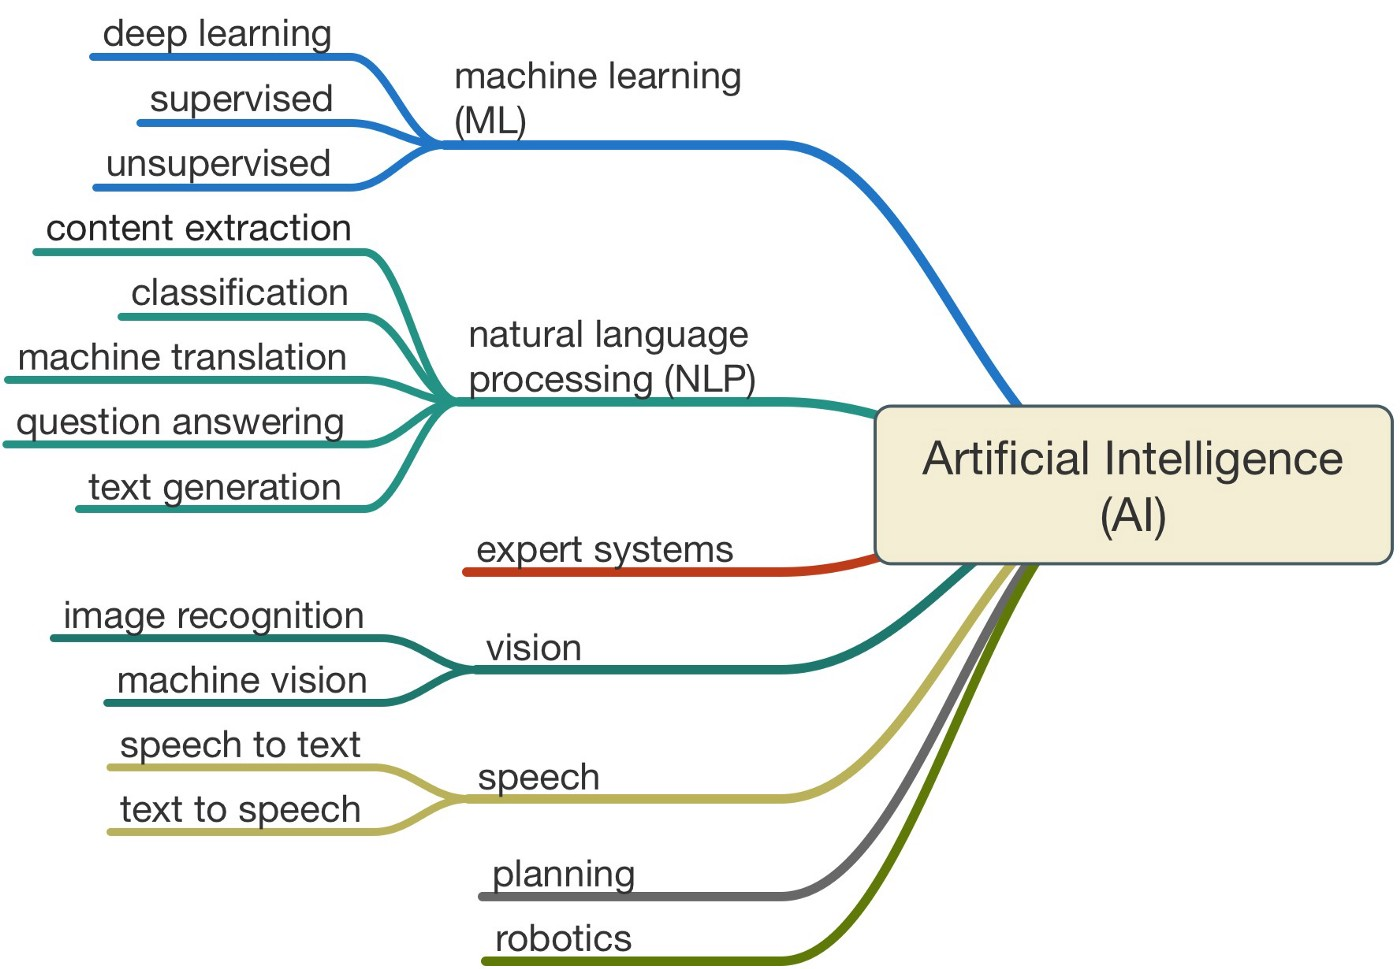
\includegraphics[width=\linewidth]{aibranches}
  \caption{applicazioni dell'IA \cite{branch}}.
  \label{fig:branches}
\end{figure}
In Figura \ref{fig:branches} vengono riportate alcune delle applicazioni di maggior successo dei \emph{Sistemi Intelligenti}.
Il settore delle Self driving Car si basa in particolare su \textbf{Machine Learning} applicato alla \textbf{Computer Vision}.
